\subsection{State}

The \textbf{World State}, referred as the \emph{state}, in its simplest
definition, is a mapping between account addresses and account states.

\begin{figure}[h]
  \centering
  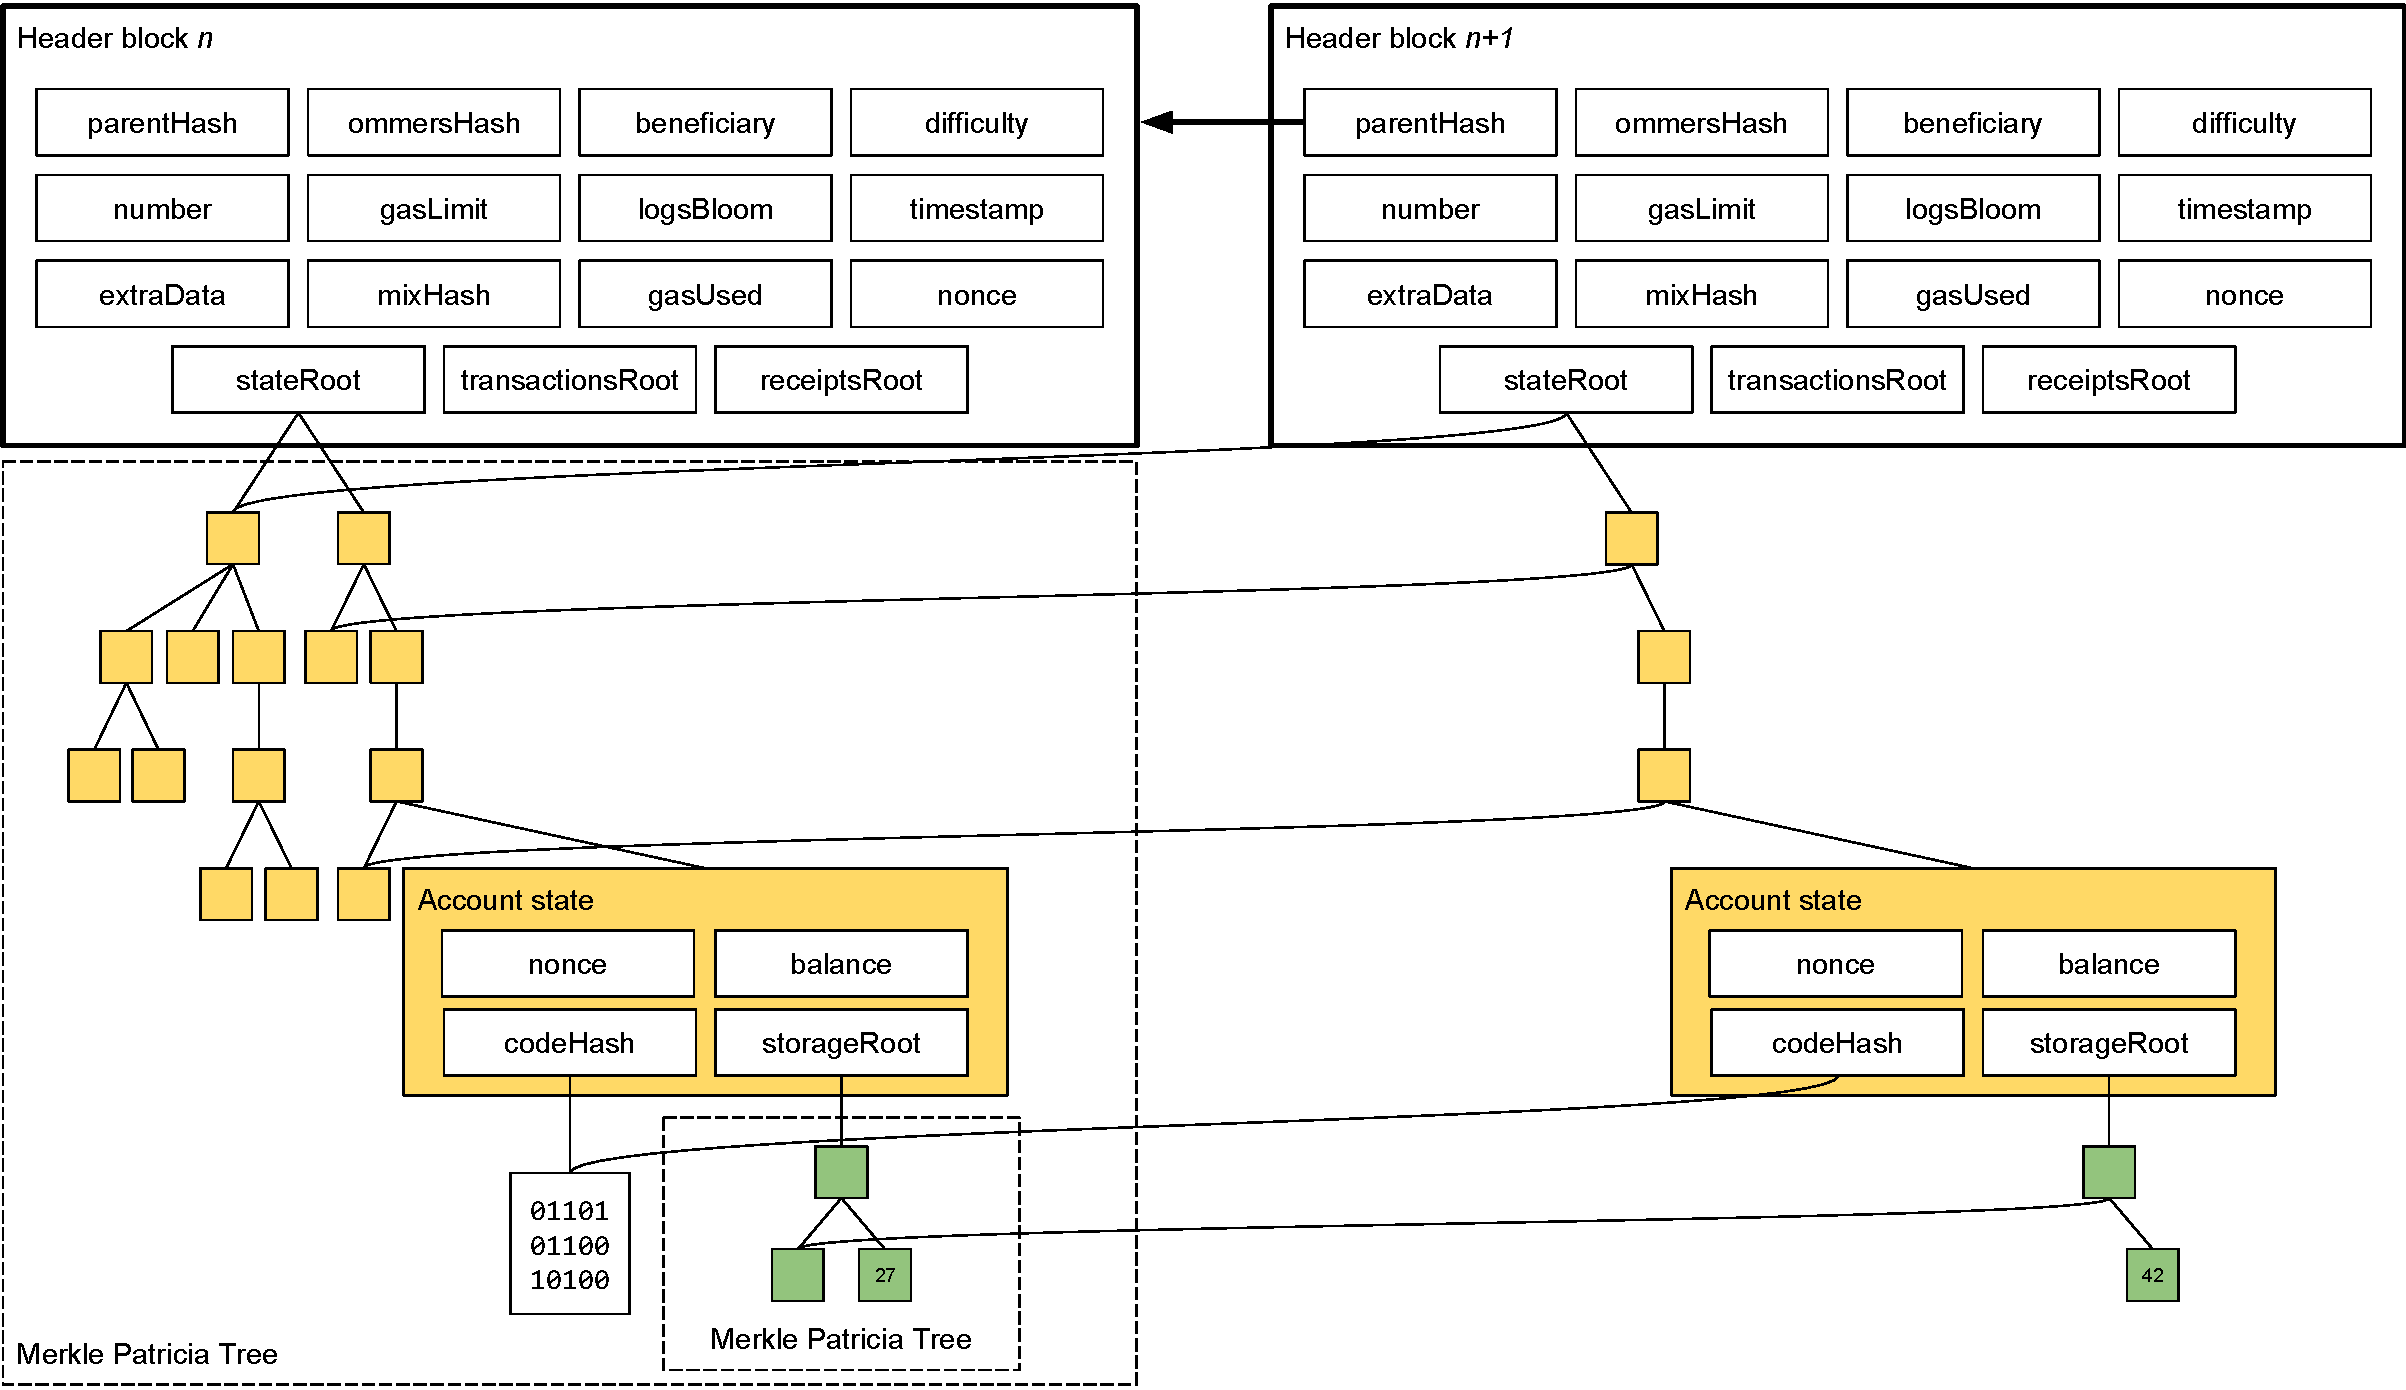
\includegraphics[width=\textwidth]{./res/img/world-state.pdf}
  \captionsource{Representation of the World State.}{Adapted from \url{https://ethereum.stackexchange.com/a/757}}
\label{fig:world-state}
\end{figure}

\autoref{fig:world-state} represents it. The block header contains 15 fields,
among which the \verb+stateRoot+, the \verb+transactionsRoot+ and the
\verb+receiptsRoot+. All these three fields are a hash\footnote{Here we intend
the Keccak 256-bit.} of the root of a Merkle Patricia tree data structure:

\begin{itemize}
  \item the \verb+stateRoot+ is the state tree, after all transactions
  are executed and finalisations applied (for a complete specification of the
  fields, refer to \cite{wood2018ethereum}), storing the mapping between account
  state and account address
  \item the \verb+transactionsRoot+ is the list of the transactions included in
  the block
  \item the \verb+receiptsRoot+ is the receipts list of the transactions
  included in the block, which shows the \emph{effect} of each transaction. In
  \cite{merklingethereum}, Vitalik Buterin\footnote{The Ethereum's founder.}
  writes that with the receipt information, someone can answer queries like "Tell
  me all instances of an event of type X (eg. a crowdfunding contract reaching
  its goal) emitted by this address in the past 30 days"
\end{itemize}

A Merkle Patricia tree is a data structure which derives from a radix tree
reducing the space complexity \cite{patriciatree}. It has a single root, each
node is the hash of its children and the leaves are the actual data, that is,
for the case of the \verb+stateRoot+, the accounts states, which in turn include
the \verb+storageRoot+, a hash of another Merkle Patricia tree representing the
storage contents of the account state.

Since each node is the hash of its children, if any data in the tree change,
recursively and correspondingly have to change all the ancestors nodes from the
changed node to the root node. This property allows us to identify uniquely a
tree having just the root node. This is worth notice because it influences
the system scalability. Briefly, we can distinguish between \emph{light nodes}
and \emph{full nodes}. The formers store just the blocks' headers, while the
latters store the entire blockchain. The tree's property we just mentioned
allows the light nodes to the validation process even without storing all the
data. This is better analyzed in \autoref{sec:scalability} talking about the
scalability.

\subsubsection{Accounts}
\label{sec:accounts}

The accounts are also called the \emph{state objects} and are essential for the
user to interact with the Ethereum blockchain via transactions.

There are two types of accounts:

\begin{itemize}
  \item the \textbf{non-contract account} (referred to as \emph{account} or
  Externally Owned Account, EOA)
  \item the \textbf{contract account} (referred to as \emph{contract}), which
  has EVM Code associated with it and is controlled by its contract code
\end{itemize}

A \emph{non-contract account} has no EVM Code associated with it and is
controlled by a private key. This type of account can send a message to another
non-contract account, that is a value transfer, or to a contract account in
order to trigger the execution of code. The state of an account is its balance.

A \emph{contract account} has EVM Code associated with it and is controlled by
it. This type of account cannot send messages or transactions on its own, but
only as a response to a trigger. The state of a contract is its balance and its
contract storage. A contract code is executed by the EVM, can manipulate its own
persistent storage and can send internal transactions (i.e. message calls) to
other contracts.
